
\input{../../2021/style/preamble4tex}
% dependencies: amsmath, amssymb, dsfont
% math spaces
\ifdefined\N
\renewcommand{\N}{\mathds{N}} % N, naturals
\else \newcommand{\N}{\mathds{N}} \fi
\newcommand{\Z}{\mathds{Z}} % Z, integers
\newcommand{\Q}{\mathds{Q}} % Q, rationals
\newcommand{\R}{\mathds{R}} % R, reals
\ifdefined\C
\renewcommand{\C}{\mathds{C}} % C, complex
\else \newcommand{\C}{\mathds{C}} \fi
\newcommand{\continuous}{\mathcal{C}} % C, space of continuous functions
\newcommand{\M}{\mathcal{M}} % machine numbers
\newcommand{\epsm}{\epsilon_m} % maximum error

% counting / finite sets
\newcommand{\setzo}{\{0, 1\}} % set 0, 1
\newcommand{\setmp}{\{-1, +1\}} % set -1, 1
\newcommand{\unitint}{[0, 1]} % unit interval

% basic math stuff
\newcommand{\xt}{\tilde x} % x tilde
\DeclareMathOperator*{\argmax}{arg\,max} % argmax
\DeclareMathOperator*{\argmin}{arg\,min} % argmin
\newcommand{\argminlim}{\mathop{\mathrm{arg\,min}}\limits} % argmax with limits
\newcommand{\argmaxlim}{\mathop{\mathrm{arg\,max}}\limits} % argmin with limits
\newcommand{\sign}{\operatorname{sign}} % sign, signum
\newcommand{\I}{\mathbb{I}} % I, indicator
\newcommand{\order}{\mathcal{O}} % O, order
\newcommand{\bigO}{\mathcal{O}} % Big-O Landau
\newcommand{\littleo}{{o}} % Little-o Landau
\newcommand{\pd}[2]{\frac{\partial{#1}}{\partial #2}} % partial derivative
\newcommand{\floorlr}[1]{\left\lfloor #1 \right\rfloor} % floor
\newcommand{\ceillr}[1]{\left\lceil #1 \right\rceil} % ceiling
\newcommand{\indep}{\perp \!\!\! \perp} % independence symbol

% sums and products
\newcommand{\sumin}{\sum\limits_{i=1}^n} % summation from i=1 to n
\newcommand{\sumim}{\sum\limits_{i=1}^m} % summation from i=1 to m
\newcommand{\sumjn}{\sum\limits_{j=1}^n} % summation from j=1 to p
\newcommand{\sumjp}{\sum\limits_{j=1}^p} % summation from j=1 to p
\newcommand{\sumik}{\sum\limits_{i=1}^k} % summation from i=1 to k
\newcommand{\sumkg}{\sum\limits_{k=1}^g} % summation from k=1 to g
\newcommand{\sumjg}{\sum\limits_{j=1}^g} % summation from j=1 to g
\newcommand{\summM}{\sum\limits_{m=1}^M} % summation from m=1 to M
\newcommand{\meanin}{\frac{1}{n} \sum\limits_{i=1}^n} % mean from i=1 to n
\newcommand{\meanim}{\frac{1}{m} \sum\limits_{i=1}^m} % mean from i=1 to n
\newcommand{\meankg}{\frac{1}{g} \sum\limits_{k=1}^g} % mean from k=1 to g
\newcommand{\meanmM}{\frac{1}{M} \sum\limits_{m=1}^M} % mean from m=1 to M
\newcommand{\prodin}{\prod\limits_{i=1}^n} % product from i=1 to n
\newcommand{\prodkg}{\prod\limits_{k=1}^g} % product from k=1 to g
\newcommand{\prodjp}{\prod\limits_{j=1}^p} % product from j=1 to p

% linear algebra
\newcommand{\one}{\bm{1}} % 1, unitvector
\newcommand{\zero}{\mathbf{0}} % 0-vector
\newcommand{\id}{\bm{I}} % I, identity
\newcommand{\diag}{\operatorname{diag}} % diag, diagonal
\newcommand{\trace}{\operatorname{tr}} % tr, trace
\newcommand{\spn}{\operatorname{span}} % span
\newcommand{\scp}[2]{\left\langle #1, #2 \right\rangle} % <.,.>, scalarproduct
\newcommand{\mat}[1]{\begin{pmatrix} #1 \end{pmatrix}} % short pmatrix command
\newcommand{\Amat}{\mathbf{A}} % matrix A
\newcommand{\Deltab}{\mathbf{\Delta}} % error term for vectors

% basic probability + stats
\renewcommand{\P}{\mathds{P}} % P, probability
\newcommand{\E}{\mathds{E}} % E, expectation
\newcommand{\var}{\mathsf{Var}} % Var, variance
\newcommand{\cov}{\mathsf{Cov}} % Cov, covariance
\newcommand{\corr}{\mathsf{Corr}} % Corr, correlation
\newcommand{\normal}{\mathcal{N}} % N of the normal distribution
\newcommand{\iid}{\overset{i.i.d}{\sim}} % dist with i.i.d superscript
\newcommand{\distas}[1]{\overset{#1}{\sim}} % ... is distributed as ...

% machine learning
\newcommand{\Xspace}{\mathcal{X}} % X, input space
\newcommand{\Yspace}{\mathcal{Y}} % Y, output space
\newcommand{\Zspace}{\mathcal{Z}} % Z, space of sampled datapoints
\newcommand{\nset}{\{1, \ldots, n\}} % set from 1 to n
\newcommand{\pset}{\{1, \ldots, p\}} % set from 1 to p
\newcommand{\gset}{\{1, \ldots, g\}} % set from 1 to g
\newcommand{\Pxy}{\mathbb{P}_{xy}} % P_xy
\newcommand{\Exy}{\mathbb{E}_{xy}} % E_xy: Expectation over random variables xy
\newcommand{\xv}{\mathbf{x}} % vector x (bold)
\newcommand{\xtil}{\tilde{\mathbf{x}}} % vector x-tilde (bold)
\newcommand{\yv}{\mathbf{y}} % vector y (bold)
\newcommand{\xy}{(\xv, y)} % observation (x, y)
\newcommand{\xvec}{\left(x_1, \ldots, x_p\right)^\top} % (x1, ..., xp)
\newcommand{\Xmat}{\mathbf{X}} % Design matrix
\newcommand{\allDatasets}{\mathds{D}} % The set of all datasets
\newcommand{\allDatasetsn}{\mathds{D}_n}  % The set of all datasets of size n
\newcommand{\D}{\mathcal{D}} % D, data
\newcommand{\Dn}{\D_n} % D_n, data of size n
\newcommand{\Dtrain}{\mathcal{D}_{\text{train}}} % D_train, training set
\newcommand{\Dtest}{\mathcal{D}_{\text{test}}} % D_test, test set
\newcommand{\xyi}[1][i]{\left(\xv^{(#1)}, y^{(#1)}\right)} % (x^i, y^i), i-th observation
\newcommand{\Dset}{\left( \xyi[1], \ldots, \xyi[n]\right)} % {(x1,y1)), ..., (xn,yn)}, data
\newcommand{\defAllDatasetsn}{(\Xspace \times \Yspace)^n} % Def. of the set of all datasets of size n
\newcommand{\defAllDatasets}{\bigcup_{n \in \N}(\Xspace \times \Yspace)^n} % Def. of the set of all datasets
\newcommand{\xdat}{\left\{ \xv^{(1)}, \ldots, \xv^{(n)}\right\}} % {x1, ..., xn}, input data
\newcommand{\ydat}{\left\{ \yv^{(1)}, \ldots, \yv^{(n)}\right\}} % {y1, ..., yn}, input data
\newcommand{\yvec}{\left(y^{(1)}, \hdots, y^{(n)}\right)^\top} % (y1, ..., yn), vector of outcomes
\newcommand{\greekxi}{\xi} % Greek letter xi
\renewcommand{\xi}[1][i]{\xv^{(#1)}} % x^i, i-th observed value of x
\newcommand{\yi}[1][i]{y^{(#1)}} % y^i, i-th observed value of y
\newcommand{\xivec}{\left(x^{(i)}_1, \ldots, x^{(i)}_p\right)^\top} % (x1^i, ..., xp^i), i-th observation vector
\newcommand{\xj}{\xv_j} % x_j, j-th feature
\newcommand{\xjvec}{\left(x^{(1)}_j, \ldots, x^{(n)}_j\right)^\top} % (x^1_j, ..., x^n_j), j-th feature vector
\newcommand{\phiv}{\mathbf{\phi}} % Basis transformation function phi
\newcommand{\phixi}{\mathbf{\phi}^{(i)}} % Basis transformation of xi: phi^i := phi(xi)

%%%%%% ml - models general
\newcommand{\lamv}{\bm{\lambda}} % lambda vector, hyperconfiguration vector
\newcommand{\Lam}{\Lambda}	 % Lambda, space of all hpos
% Inducer / Inducing algorithm
\newcommand{\preimageInducer}{\left(\defAllDatasets\right)\times\Lam} % Set of all datasets times the hyperparameter space
\newcommand{\preimageInducerShort}{\allDatasets\times\Lam} % Set of all datasets times the hyperparameter space
% Inducer / Inducing algorithm
\newcommand{\ind}{\mathcal{I}} % Inducer, inducing algorithm, learning algorithm

% continuous prediction function f
\newcommand{\ftrue}{f_{\text{true}}}  % True underlying function (if a statistical model is assumed)
\newcommand{\ftruex}{\ftrue(\xv)} % True underlying function (if a statistical model is assumed)
\newcommand{\fx}{f(\xv)} % f(x), continuous prediction function
\newcommand{\fdomains}{f: \Xspace \rightarrow \R^g} % f with domain and co-domain
\newcommand{\Hspace}{\mathcal{H}} % hypothesis space where f is from
\newcommand{\Hall}{\mathcal{H}_{\text{all}}} % unrestricted hypothesis space
\newcommand{\fbayes}{f^{\ast}} % Bayes-optimal model
\newcommand{\fxbayes}{f^{\ast}(\xv)} % Bayes-optimal model
\newcommand{\fkx}[1][k]{f_{#1}(\xv)} % f_j(x), discriminant component function
\newcommand{\fhspace}{\hat f_{\Hspace}} % fhat_H
\newcommand{\fh}{\hat{f}} % f hat, estimated prediction function
\newcommand{\fxh}{\fh(\xv)} % fhat(x)
\newcommand{\fxt}{f(\xv ~|~ \thetav)} % f(x | theta)
\newcommand{\fxi}{f\left(\xv^{(i)}\right)} % f(x^(i))
\newcommand{\fxih}{\hat{f}\left(\xv^{(i)}\right)} % f(x^(i))
\newcommand{\fxit}{f\big(\xv^{(i)} ~|~ \thetav\big)} % f(x^(i) | theta)
\newcommand{\fhD}{\fh_{\D}} % fhat_D, estimate of f based on D
\newcommand{\fhDtrain}{\fh_{\Dtrain}} % fhat_Dtrain, estimate of f based on D
\newcommand{\fhDnlam}{\fh_{\Dn, \lamv}} %model learned on Dn with hp lambda
\newcommand{\fhDlam}{\fh_{\D, \lamv}} %model learned on D with hp lambda
\newcommand{\fhDnlams}{\fh_{\Dn, \lamv^\ast}} %model learned on Dn with optimal hp lambda
\newcommand{\fhDlams}{\fh_{\D, \lamv^\ast}} %model learned on D with optimal hp lambda

% discrete prediction function h
\newcommand{\hx}{h(\xv)} % h(x), discrete prediction function
\newcommand{\hh}{\hat{h}} % h hat
\newcommand{\hxh}{\hat{h}(\xv)} % hhat(x)
\newcommand{\hxt}{h(\xv | \thetav)} % h(x | theta)
\newcommand{\hxi}{h\left(\xi\right)} % h(x^(i))
\newcommand{\hxit}{h\left(\xi ~|~ \thetav\right)} % h(x^(i) | theta)
\newcommand{\hbayes}{h^{\ast}} % Bayes-optimal classification model
\newcommand{\hxbayes}{h^{\ast}(\xv)} % Bayes-optimal classification model

% yhat
\newcommand{\yh}{\hat{y}} % yhat for prediction of target
\newcommand{\yih}{\hat{y}^{(i)}} % yhat^(i) for prediction of ith targiet
\newcommand{\resi}{\yi- \yih}

% theta
\newcommand{\thetah}{\hat{\theta}} % theta hat
\newcommand{\thetav}{\bm{\theta}} % theta vector
\newcommand{\thetavh}{\bm{\hat\theta}} % theta vector hat
\newcommand{\thetat}[1][t]{\thetav^{[#1]}} % theta^[t] in optimization
\newcommand{\thetatn}[1][t]{\thetav^{[#1 +1]}} % theta^[t+1] in optimization
\newcommand{\thetahDnlam}{\thetavh_{\Dn, \lamv}} %theta learned on Dn with hp lambda
\newcommand{\thetahDlam}{\thetavh_{\D, \lamv}} %theta learned on D with hp lambda
\newcommand{\mint}{\min_{\thetav \in \Theta}} % min problem theta
\newcommand{\argmint}{\argmin_{\thetav \in \Theta}} % argmin theta

% densities + probabilities
% pdf of x
\newcommand{\pdf}{p} % p
\newcommand{\pdfx}{p(\xv)} % p(x)
\newcommand{\pixt}{\pi(\xv~|~ \thetav)} % pi(x|theta), pdf of x given theta
\newcommand{\pixit}[1][i]{\pi\left(\xi[#1] ~|~ \thetav\right)} % pi(x^i|theta), pdf of x given theta
\newcommand{\pixii}[1][i]{\pi\left(\xi[#1]\right)} % pi(x^i), pdf of i-th x

% pdf of (x, y)
\newcommand{\pdfxy}{p(\xv,y)} % p(x, y)
\newcommand{\pdfxyt}{p(\xv, y ~|~ \thetav)} % p(x, y | theta)
\newcommand{\pdfxyit}{p\left(\xi, \yi ~|~ \thetav\right)} % p(x^(i), y^(i) | theta)

% pdf of x given y
\newcommand{\pdfxyk}[1][k]{p(\xv | y= #1)} % p(x | y = k)
\newcommand{\lpdfxyk}[1][k]{\log p(\xv | y= #1)} % log p(x | y = k)
\newcommand{\pdfxiyk}[1][k]{p\left(\xi | y= #1 \right)} % p(x^i | y = k)

% prior probabilities
\newcommand{\pik}[1][k]{\pi_{#1}} % pi_k, prior
\newcommand{\pih}{\hat{\pi}} % pi hat, estimated prior (binary classification)
\newcommand{\pikh}[1][k]{\hat{\pi}_{#1}} % pi_k hat, estimated prior
\newcommand{\lpik}[1][k]{\log \pi_{#1}} % log pi_k, log of the prior
\newcommand{\pit}{\pi(\thetav)} % Prior probability of parameter theta

% posterior probabilities
\newcommand{\post}{\P(y = 1 ~|~ \xv)} % P(y = 1 | x), post. prob for y=1
\newcommand{\postk}[1][k]{\P(y = #1 ~|~ \xv)} % P(y = k | y), post. prob for y=k
\newcommand{\pidomains}{\pi: \Xspace \rightarrow \unitint} % pi with domain and co-domain
\newcommand{\pibayes}{\pi^{\ast}} % Bayes-optimal classification model
\newcommand{\pixbayes}{\pi^{\ast}(\xv)} % Bayes-optimal classification model
\newcommand{\piastxtil}{\pi^{\ast}(\xtil)} % Bayes-optimal classification model
\newcommand{\piastkxtil}{\pi^{\ast}_k(\xtil)} % Bayes-optimal classification model for k-th class
\newcommand{\pix}{\pi(\xv)} % pi(x), P(y = 1 | x)
\newcommand{\piv}{\bm{\pi}} % pi, bold, as vector
\newcommand{\pikx}[1][k]{\pi_{#1}(\xv)} % pi_k(x), P(y = k | x)
\newcommand{\pikxt}[1][k]{\pi_{#1}(\xv ~|~ \thetav)} % pi_k(x | theta), P(y = k | x, theta)
\newcommand{\pixh}{\hat \pi(\xv)} % pi(x) hat, P(y = 1 | x) hat
\newcommand{\pikxh}[1][k]{\hat \pi_{#1}(\xv)} % pi_k(x) hat, P(y = k | x) hat
\newcommand{\pixih}{\hat \pi(\xi)} % pi(x^(i)) with hat
\newcommand{\pikxih}[1][k]{\hat \pi_{#1}(\xi)} % pi_k(x^(i)) with hat
\newcommand{\pdfygxt}{p(y ~|~\xv, \thetav)} % p(y | x, theta)
\newcommand{\pdfyigxit}{p\left(\yi ~|~\xi, \thetav\right)} % p(y^i |x^i, theta)
\newcommand{\lpdfygxt}{\log \pdfygxt } % log p(y | x, theta)
\newcommand{\lpdfyigxit}{\log \pdfyigxit} % log p(y^i |x^i, theta)

% probabilistic
\newcommand{\bayesrulek}[1][k]{\frac{\P(\xv | y= #1) \P(y= #1)}{\P(\xv)}} % Bayes rule
\newcommand{\muv}{\bm{\mu}} % expectation vector of Gaussian
\newcommand{\muk}[1][k]{\bm{\mu_{#1}}} % mean vector of class-k Gaussian (discr analysis)
\newcommand{\mukh}[1][k]{\bm{\hat{\mu}_{#1}}} % estimated mean vector of class-k Gaussian (discr analysis)

% residual and margin
\newcommand{\rx}{r(\xv)} % residual 
\newcommand{\eps}{\epsilon} % residual, stochastic
\newcommand{\epsv}{\bm{\epsilon}} % residual, stochastic, as vector
\newcommand{\epsi}{\epsilon^{(i)}} % epsilon^i, residual, stochastic
\newcommand{\epsh}{\hat{\epsilon}} % residual, estimated
\newcommand{\epsvh}{\hat{\epsv}} % residual, estimated, vector
\newcommand{\yf}{y \fx} % y f(x), margin
\newcommand{\yfi}{\yi \fxi} % y^i f(x^i), margin
\newcommand{\Sigmah}{\hat \Sigma} % estimated covariance matrix
\newcommand{\Sigmahj}{\hat \Sigma_j} % estimated covariance matrix for the j-th class
\newcommand{\nux}{\nu(\xv)} % nu(x) = y * f(x)

% ml - loss, risk, likelihood
\newcommand{\Lyf}{L\left(y, f\right)} % L(y, f), loss function
% \newcommand{\Lypi}{L\left(y, \pi\right)} % L(y, pi), loss function
\newcommand{\Lxy}{L\left(y, \fx\right)} % L(y, f(x)), loss function
\newcommand{\Lxyi}{L\left(\yi, \fxi\right)} % loss of observation
\newcommand{\Lxyt}{L\left(y, \fxt\right)} % loss with f parameterized
\newcommand{\Lxyit}{L\left(\yi, \fxit\right)} % loss of observation with f parameterized
\newcommand{\Lxym}{L\left(\yi, f\left(\bm{\tilde{x}}^{(i)} ~|~ \thetav\right)\right)} % loss of observation with f parameterized
\newcommand{\Lpixy}{L\left(y, \pix\right)} % loss in classification
% \newcommand{\Lpiy}{L\left(y, \pi\right)} % loss in classification
\newcommand{\Lpiv}{L\left(y, \piv\right)} % loss in classification
\newcommand{\Lpixyi}{L\left(\yi, \pixii\right)} % loss of observation in classification
\newcommand{\Lpixyt}{L\left(y, \pixt\right)} % loss with pi parameterized
\newcommand{\Lpixyit}{L\left(\yi, \pixit\right)} % loss of observation with pi parameterized
% \newcommand{\Lhy}{L\left(y, h\right)} % L(y, h), loss function on discrete classes
\newcommand{\Lhxy}{L\left(y, \hx\right)} % L(y, h(x)), loss function on discrete classes
\newcommand{\Lr}{L\left(r\right)} % L(r), loss defined on residual (reg) / margin (classif)
\newcommand{\lone}{|y - \fx|} % L1 loss
\newcommand{\ltwo}{\left(y - \fx\right)^2} % L2 loss
\newcommand{\lbernoullimp}{\ln(1 + \exp(-y \cdot \fx))} % Bernoulli loss for -1, +1 encoding
\newcommand{\lbernoullizo}{- y \cdot \fx + \log(1 + \exp(\fx))} % Bernoulli loss for 0, 1 encoding
\newcommand{\lcrossent}{- y \log \left(\pix\right) - (1 - y) \log \left(1 - \pix\right)} % cross-entropy loss
\newcommand{\lbrier}{\left(\pix - y \right)^2} % Brier score
\newcommand{\risk}{\mathcal{R}} % R, risk
\newcommand{\riskbayes}{\mathcal{R}^\ast}
\newcommand{\riskf}{\risk(f)} % R(f), risk
\newcommand{\riskdef}{\E_{y|\xv}\left(\Lxy \right)} % risk def (expected loss)
\newcommand{\riskt}{\mathcal{R}(\thetav)} % R(theta), risk
\newcommand{\riske}{\mathcal{R}_{\text{emp}}} % R_emp, empirical risk w/o factor 1 / n
\newcommand{\riskeb}{\bar{\mathcal{R}}_{\text{emp}}} % R_emp, empirical risk w/ factor 1 / n
\newcommand{\riskef}{\riske(f)} % R_emp(f)
\newcommand{\risket}{\mathcal{R}_{\text{emp}}(\thetav)} % R_emp(theta)
\newcommand{\riskr}{\mathcal{R}_{\text{reg}}} % R_reg, regularized risk
\newcommand{\riskrt}{\mathcal{R}_{\text{reg}}(\thetav)} % R_reg(theta)
\newcommand{\riskrf}{\riskr(f)} % R_reg(f)
\newcommand{\riskrth}{\hat{\mathcal{R}}_{\text{reg}}(\thetav)} % hat R_reg(theta)
\newcommand{\risketh}{\hat{\mathcal{R}}_{\text{emp}}(\thetav)} % hat R_emp(theta)
\newcommand{\LL}{\mathcal{L}} % L, likelihood
\newcommand{\LLt}{\mathcal{L}(\thetav)} % L(theta), likelihood
\newcommand{\LLtx}{\mathcal{L}(\thetav | \xv)} % L(theta|x), likelihood
\newcommand{\logl}{\ell} % l, log-likelihood
\newcommand{\loglt}{\logl(\thetav)} % l(theta), log-likelihood
\newcommand{\logltx}{\logl(\thetav | \xv)} % l(theta|x), log-likelihood
\newcommand{\errtrain}{\text{err}_{\text{train}}} % training error
\newcommand{\errtest}{\text{err}_{\text{test}}} % test error
\newcommand{\errexp}{\overline{\text{err}_{\text{test}}}} % avg training error

% lm
\newcommand{\thx}{\thetav^\top \xv} % linear model
\newcommand{\olsest}{(\Xmat^\top \Xmat)^{-1} \Xmat^\top \yv} % OLS estimator in LM

% ml - Gaussian Process

\newcommand{\fvec}{[f(\xi[1]), \dots, f(\xi[n])]} % {f(x1), ..., f(xn)}
\newcommand{\fv}{\mathbf{f}} % bold f, function vector 
\newcommand{\mv}{\mathbf{m}} % bold m, GP mean vector 
\newcommand{\kv}{\mathbf{k}} % bold k, kernel mat partition 
\newcommand{\kcc}{k(\cdot, \cdot)} % k(.,.), kernel for arbitrary inputs 
\newcommand{\kxij}[2]{k(\xi, \xi[j])} % k(xi, xj), cov of x_i, x_j
\newcommand{\Kmat}{\mathbf{K}} % K, kernel mat
\newcommand{\Nmk}{\normal(\mv, \Kmat)} % n(m,K), Gaussian w/ mean vec, cov mat
\newcommand{\Nzk}{\normal(\zero, \Kmat)} % n(0,K), zero-mean Gaussian
\newcommand{\GPmk}{\mathcal{GP}(m(\cdot), \kcc)} % GP(m(.), k(.,.)), GP definition
\newcommand{\GPzk}{\mathcal{GP}(\zero, \kcc)} % GP(0, k(.,.)), zero-mean GP
\newcommand{\Xsubset}{\bm{X}} % bold X, finite subset from xspace
\newcommand{\fX}{f(\Xsubset)} % f(X), function vector of finite subset
\newcommand{\kXX}{k(\Xsubset, \Xsubset)} % k(X,X), cov for finite subset
\newcommand{\mX}{m(\Xsubset)} % m(X), mean for finite subset
\newcommand{\ls}{\ell} % length-scale
\newcommand{\xxtnorm}{\| \xv - \xtil\|} % ||x - xtilde||

% GP prediction
\newcommand{\xs}{\xv_\ast} % x_*, test obs features
\newcommand{\ys}{\yv_\ast} % y_*, test obs target
\newcommand{\fs}{\fv_\ast} % f_*, test obs fun vector
\newcommand{\Xs}{\Xmat_\ast} % X_*, test design matrix
\newcommand{\ks}{\kv_{\ast}} % k_*, cov vec of new obs with x
\newcommand{\kss}{\kv_{\ast \ast}} % k_**, cov vec of new obs
\newcommand{\Ks}{\Kmat_{\ast}} % K_*, cov mat of new obs with x
\newcommand{\Kss}{\Kmat_{\ast \ast}} % K_**, cov mat of new obs
\newcommand{\Kinv}{\Kmat^{-1}} % K^-1, inverse cov mat
\newcommand{\Ky}{\Kmat_y} % K_y, cov mat of y



\begin{document}

\lecturechapter{10}{Gaussian Processes}
\lecture{Fortgeschrittene Computerintensive Methoden}


\begin{vbframe}{Weight-Space View}

\begin{itemize}
  \item Until now we considered a hypothesis space $\Hspace$ of parameterized functions $\fxt$ (in particular, the space of linear functions). 
  \item Using Bayesian inference, we derived distributions for $\thetab$ after having observed data $\D$. 
  \item Prior believes about the parameter are expressed via a prior distribution $q(\thetab)$, which is updated according to Bayes' rule 

  $$
  \underbrace{p(\thetab | \Xmat, \ydat)}_{\text{posterior}} = \frac{\overbrace{p(\ydat | \Xmat, \thetab)}^{\text{likelihood}}\overbrace{q(\thetab)}^{\text{prior}}}{\underbrace{p(\ydat|\Xmat)}_{\text{marginal}}}. 
  $$
\end{itemize}

\end{vbframe}


\begin{vbframe}{Function-space View}

Let us change our point of view: 

\begin{itemize}
  \item Instead of \enquote{searching} for a parameter  $\thetab$ in the parameter space, we directly search in a space of \enquote{allowed} functions $\Hspace$.  
  \item We still use Bayesian inference, but instead specifying a prior distribution over a parameter, we specify a prior distribution \textbf{over functions} and update it according to the data points we have observed. 
\end{itemize}

\framebreak 

Intuitively, imagine we could draw a huge number of functions from some prior distribution over functions $^{(*)}$. 

\begin{figure}
  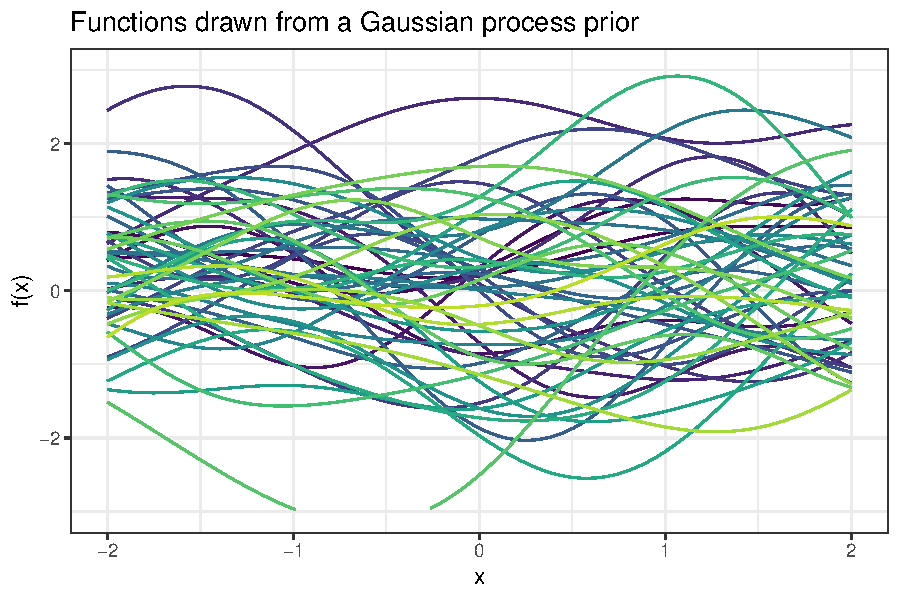
\includegraphics[width=0.8\textwidth]{figure_man/gp-sample/gp-sample-1-1.pdf}
\end{figure}

\vspace*{-0.5cm}

\begin{footnotesize}
  $^{(*)}$ We will see in a minute how distributions over functions can be specified. 
\end{footnotesize}

\framebreak 

\foreach \x in{1,2,3} {
    After observing some data points, we are only allowed to sample those functions, that are consistent with the data. \\
  \begin{figure}
    \includegraphics[width=0.8\textwidth]{figure_man/gp-sample/gp-sample-2-\x.pdf}
  \end{figure}
}

\framebreak 

As we observe more and more data points, the variety of functions consistent with the data shrinks. 
  \begin{figure}
    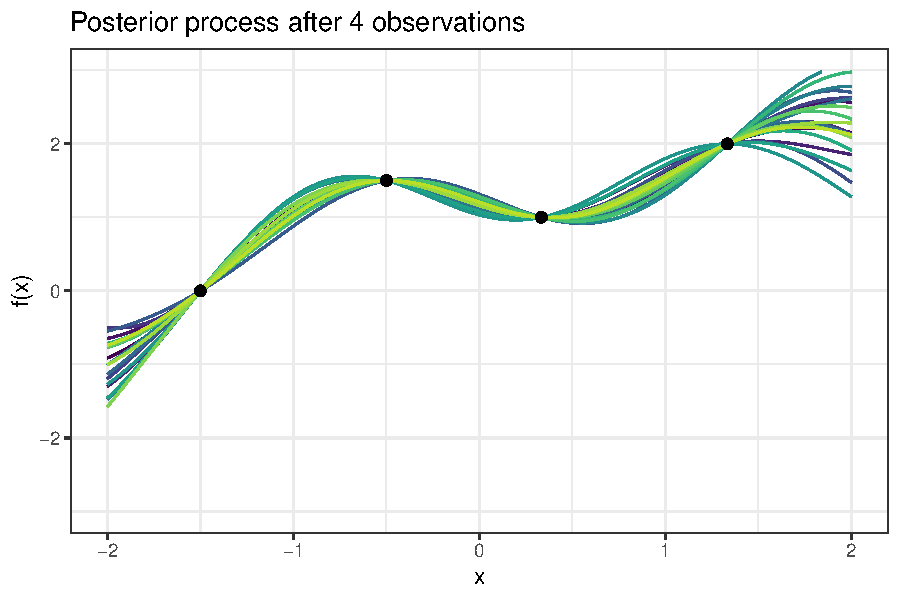
\includegraphics[width=0.8\textwidth]{figure_man/gp-sample/gp-sample-2-4.pdf}
  \end{figure}

\framebreak 

Inutitively, there is something like \enquote{mean} and a \enquote{variance} of a distribution over functions. 

  \begin{figure}
    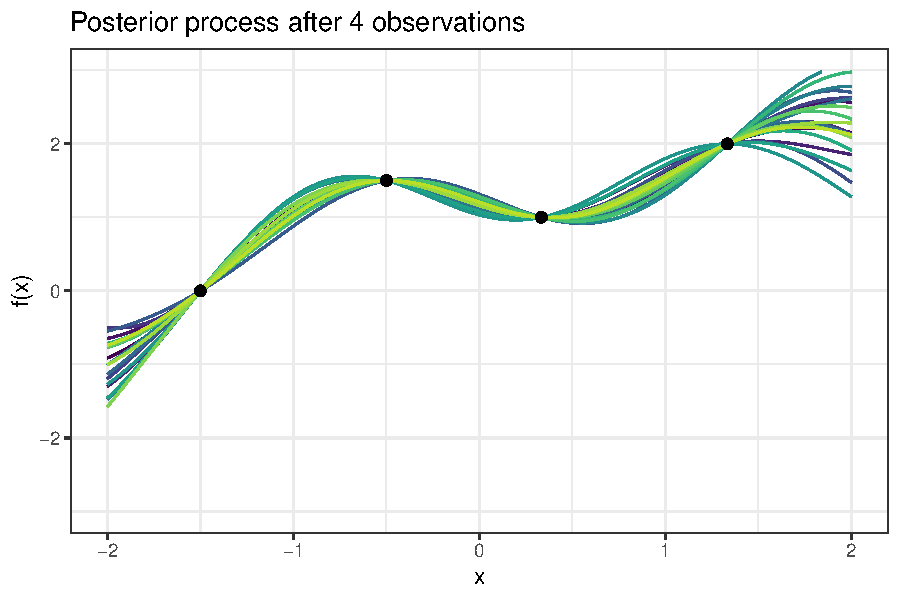
\includegraphics[width=0.8\textwidth]{figure_man/gp-sample/gp-sample-2-4.pdf}
  \end{figure}

\end{vbframe}

\begin{frame}{Weight-space vs. Function-space View}

\begin{table}
  \begin{tabular}{cc}
  \textbf{Weight-Space View} & \textbf{Function-Space View} \vspace{4mm}\\ 
  Parameterize functions & \vspace{1mm}\\
  \footnotesize Example: $\fxt = \thetab^\top \xv$ & \vspace{3mm}\\
  Define distributions on $\thetab$ & Define distributions on $f$ \vspace{4mm}\\
  Inference in parameter space $\Theta$ & Inference in function space $\Hspace$
  \end{tabular}
\end{table}  

\lz

Next, we will see how we can define distributions over functions mathematically. 


\end{frame}

\section{Distributions on Functions}

\begin{vbframe}{Discrete Functions}

For simplicity, let us consider functions with finite domains first. 

\lz 


Let $\mathcal{X} = \left\{\xv^{(1)}, \dots , \xv^{(n)}\right\}$ be a finite set of elements and $\Hspace$ the set of all functions from $\mathcal{X} \to \R$.

\lz

Since the domain of any $h(.) \in \Hspace$ has only $n$ elements, we can represent the function $h(.)$ compactly as a $n$-dimensional vector $$\bm{h} = \left[h\left(\xv^{(1)}\right), \dots, h\left(\xv^{(n)}\right)\right].$$
\end{vbframe}


\begin{frame}{Discrete Functions}

\textbf{Example 1:} Let us consider $h: \Xspace \to \Yspace$ where the input space consists of \textbf{two} points $\Xspace = \{0, 1\}$. 

\lz 

Examples for functions that live in this space: 

\begin{figure}[h]
\foreach \x in{1,2,3} {
  \includegraphics<\x>[width=0.7\linewidth]{figure_man/discrete/example_2_\x.pdf} \par
}
\end{figure}


\end{frame}

\begin{frame}{Discrete Functions}

\textbf{Example 2:} Let us consider $h: \Xspace \to \Yspace$ where the input space consists of \textbf{five} points $\Xspace = \{0, 0.25, 0.5, 0.75, 1\}$.

\lz 

Examples for functions that live in this space: 

\begin{figure}[h]
\foreach \x in{1,2,3} {
  \includegraphics<\x>[width=0.7\linewidth]{figure_man/discrete/example_5_\x.pdf}\par
}
\end{figure}

\end{frame}


\begin{frame}{Discrete Functions}

\textbf{Example 3:} Let us consider $h: \Xspace \to \Yspace$ where the input space consists of \textbf{ten} points. 

\lz 

Examples for functions that live in this space: 

\begin{figure}[h]
\foreach \x in{1,2,3} {
  \includegraphics<\x>[width=0.7\linewidth]{figure_man/discrete/example_10_\x.pdf}\par
}
\end{figure}

\end{frame}


\begin{vbframe}{Distributions on Discrete Functions}

\vspace*{0.5cm}

One natural way to specify a probability function on discrete function $h \in \Hspace$ is to use the vector representation 
$$
  \bm{h} = \left[h\left(\xi[1]\right), h\left(\xi[2]\right), \dots, h\left(\xi[n]\right)\right]
$$ 


of the function.

\lz

Let us see $\bm{h}$ as a $n$-dimensional random variable. We will further assume the following normal distribution: 

$$
  \bm{h} \sim \mathcal{N}\left(\bm{m}, \bm{K}\right).
$$ 

\textbf{Note: } For now, we set $\bm{m} = \bm{0}$ and take the covariance matrix $\bm{K}$ as given. We will see later how they are chosen / estimated. 

\end{vbframe}

\begin{frame}{Discrete Functions}

\textbf{Example 1 (continued):} Let $h: \Xspace \to \Yspace$ be a function that is defined on \textbf{two} points $\Xspace$. We sample functions by sampling from a two-dimensional normal variable

$$
\bm{h} = [h(1), h(2)] \sim \mathcal{N}(\bm{m}, \bm{K})
$$


\begin{figure}[H]
\foreach \x in{1,2,3} {
  \includegraphics<\x>[width=0.4\linewidth]{figure_man/discrete/example_norm_2_\x-a.pdf} ~  \includegraphics<\x>[width=0.4\linewidth]{figure_man/discrete/example_norm_2_\x-b.pdf} 
} \par
\begin{footnotesize}
In this example, $m = (0, 0)$ and $K = \begin{pmatrix} 1 & 0.5 \\ 0.5 & 1 \end{pmatrix}$. 
\end{footnotesize}
\end{figure}

\end{frame}


\begin{frame}{Discrete Functions}

\textbf{Example 2 (continued):} Let us consider $h: \Xspace \to \Yspace$ where the input space consists of \textbf{five} points. We sample functions by sampling from a five-dimensional normal variable


$$
\bm{h} = [h(1), h(2), h(3), h(4), h(5)] \sim \mathcal{N}(\bm{m}, \bm{K})
$$

\begin{figure}[h]
\foreach \x in{1,2,3} {
  \includegraphics<\x>[width=0.4\linewidth]{figure_man/discrete/example_norm_5_\x-a.pdf} ~  \includegraphics<\x>[width=0.4\linewidth]{figure_man/discrete/example_norm_5_\x-b.pdf}
}
\end{figure}

\end{frame}

\begin{frame}{Discrete Functions}

\textbf{Example 3 (continued):} Let us consider $h: \Xspace \to \Yspace$ where the input space consists of \textbf{ten} points. We sample functions by sampling from ten-dimensional normal variable

$$
\bm{h} = [h(1), h(2), \dots, h(10)] \sim \mathcal{N}(\bm{m}, \bm{K})
$$

\begin{figure}[h]
\foreach \x in{1,2,3} {
  \includegraphics<\x>[width=0.4\linewidth]{figure_man/discrete/example_norm_10_\x-a.pdf} ~  \includegraphics<\x>[width=0.4\linewidth]{figure_man/discrete/example_norm_10_\x-b.pdf}
}
\end{figure}

\end{frame}


\begin{vbframe}{Role of the Covariance Function}

Note that the covariance controls the \enquote{shape} of the drawn function. Consider two extreme cases where function values are

\begin{enumerate}
  \item[a)] strongly correlated: $\bm{K} = \begin{footnotesize}\begin{pmatrix} 1 & 0.99 & \dots & 0.99 \\
  0.99 & 1 & \dots & 0.99 \\
  0.99 & 0.99 & \ddots & 0.99 \\
  0.99 & \dots & 0.99 & 1 \end{pmatrix}\end{footnotesize}$
  \item[b)] uncorrelated: $\bm{K} = \id$
\end{enumerate}

\begin{figure}
  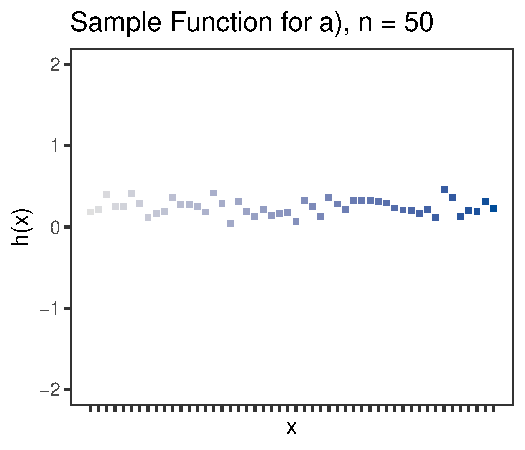
\includegraphics[width=0.35\linewidth]{figure_man/discrete/example_extreme_50-1.pdf} ~~  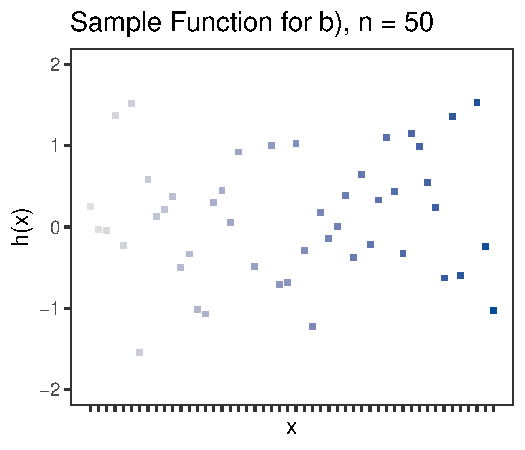
\includegraphics[width=0.35\linewidth]{figure_man/discrete/example_extreme_50-2.pdf}
\end{figure}


\framebreak 

\begin{itemize}
  \item \enquote{Meaningful} functions (on a numeric space $\Xspace$) may be characterized by a spatial property: \vspace*{0.2cm}
  \begin{itemize}
    \item[] If two points $\xi, \xi[j]$ are close in $\Xspace$-space, their function values $f(\xi), f(\xi[j])$ should be close in $\Yspace$-space. 
  \end{itemize} \vspace*{0.2cm}
  In other words: If they are close in $\Xspace$-space, their functions values should be \textbf{correlated}! \vspace*{0.4cm}
  \item We can enforce that by choosing a covariance function with  
  $$
    \bm{K}_{ij} \text{ high, if } \xi[i], \xi[j] \text{ close.}
  $$

  \framebreak 

  \item We can compute the entries of the covariance matrix by a function that is based on the distance between $\xi, \xi[j]$, for example: 
  
  \vspace*{0.2cm}
  \begin{enumerate}
    \item[c)] Spatial correlation: \begin{footnotesize}$K_{ij} = k(\xi[i], \xi[j]) = \exp\left(-\frac{1}{2}\left|\xi - \xi[j]\right|^2\right)$\end{footnotesize}
  \end{enumerate}
  
\begin{figure}
  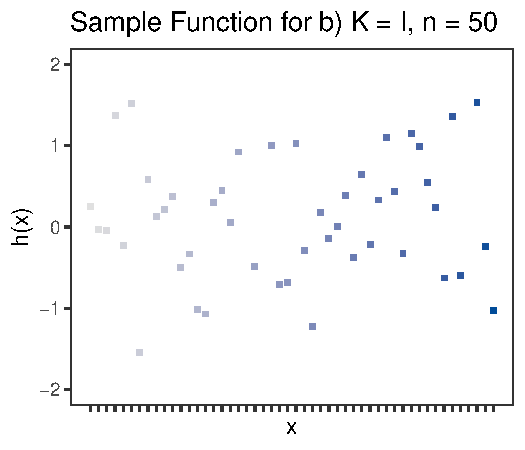
\includegraphics[width=0.45\linewidth]{figure_man/discrete/example_extreme_50-4.pdf} ~~  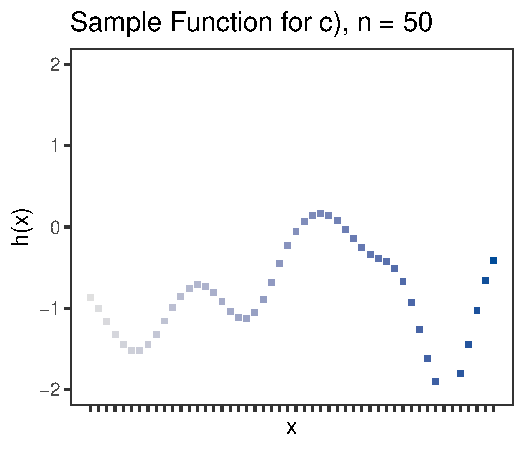
\includegraphics[width=0.45\linewidth]{figure_man/discrete/example_extreme_50-3.pdf}
\end{figure}

\end{itemize}

\begin{footnotesize}
\textbf{Note}: $k(\cdot,\cdot)$ is known as the \textbf{covariance function} or \textbf{kernel}. It will be studied in more detail later on.
\end{footnotesize}

\end{vbframe}




% \begin{vbframe}
% \begin{figure}
% 	\centering
% 	\includegraphics{figure_man/discrete/sample2.png} \\
% 	\begin{footnotesize} If we sample again, we get another function. 
% 	\end{footnotesize}
% \end{figure}


% However, we are usually interested in functions with infinite domain size. 

% \lz 

% This idea is extended to infinite domain size via \textbf{Gaussian processes}. 

% \end{vbframe}


\section{Gaussian Processes}

\begin{vbframe}{From Discrete to Continuous Functions}

\begin{itemize}
  \item We defined distributions on functions with discrete domain by defining a Gaussian on the vector of the respective function values 
  $$
    \mathbf{h} = [h(\xi[1]), h(\xi[2]), \dots, h(\xi[n])] \sim \mathcal{N}(\bm{m}, \bm{K})
  $$

  \item We can do this for $n \to \infty$ (as \enquote{granular} as we want)
  \begin{figure}
    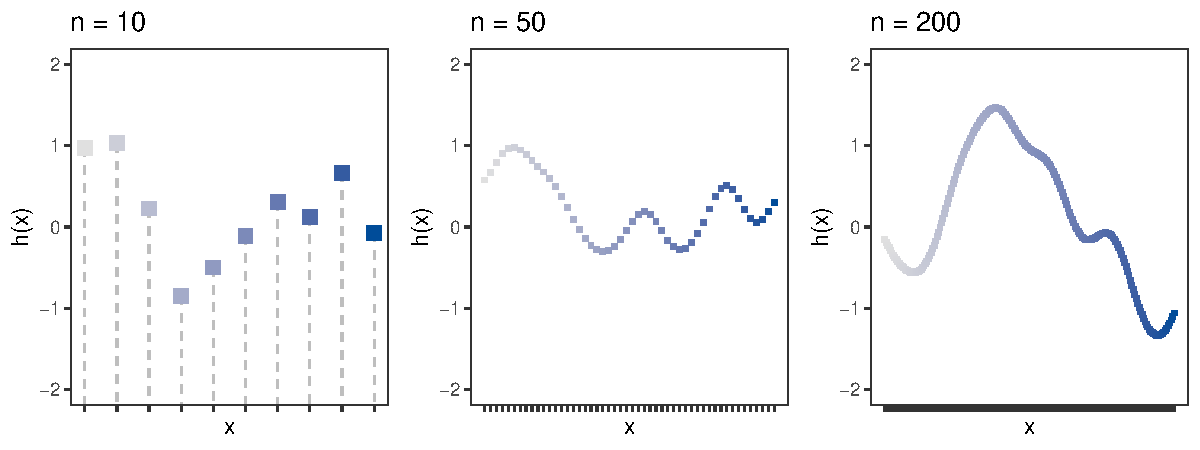
\includegraphics[width = 0.9\textwidth]{figure_man/discrete/example_limit.pdf}
  \end{figure}
\end{itemize}

\end{vbframe}

\begin{frame}{From Discrete to Continuous Functions}


\begin{itemize}
  \item No matter how large $n$ is, we are still considering a function over a discrete domain. 
  \item How can we extend our definition to functions with \textbf{continuous domain} $\Xspace \subset \R$?
\end{itemize}

\end{frame}


\begin{frame}{Gaussian Processes: Intuition}

\begin{itemize}
  \only<1>{
    \item Intuitively, a function $f$ drawn from \textbf{Gaussian process} can be understood as an \enquote{infinite} long Gaussian random vector. 
    \item It is unclear how to handle an \enquote{infinite} long Gaussian random vector!
  \lz 
  \begin{figure}
    
\includegraphics[width=0.3\textwidth]{figure_man/question.png}
  \end{figure}
  }
  \only<2-4>{
    \item Thus, it is required that for \textbf{any finite set} of inputs $\{\xi[1], \dots, \xi[n]\} \subset \Xspace$, the vector $\mathbf{f}$ has a Gaussian distribution
    $$
      \bm{f} = \left[f\left(\xi[1]\right), \dots, f\left(\xi[n]\right)\right] \sim \mathcal{N}\left(\bm{m}, \bm{K}\right),
    $$ 
    with $\bm{m}$ and $\bm{K}$ being calculated by a mean function $m(.)$ / covariance function $k(.,.)$.
    \item This property is called \textbf{Marginalization Property}. 
    \begin{figure}
      \only<2>{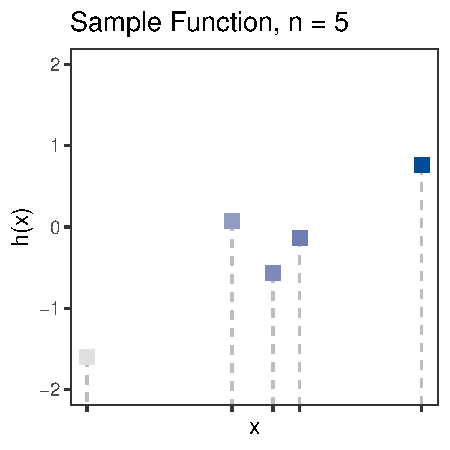
\includegraphics[width=0.4\textwidth]{figure_man/discrete/example_marginalization_5.pdf}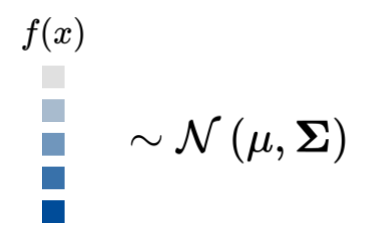
\includegraphics[width=0.5\textwidth]{figure_man/discrete/marginalization-5.png}}
      \only<3>{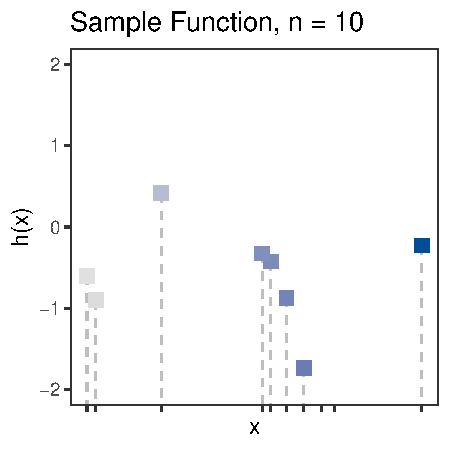
\includegraphics[width=0.4\textwidth]{figure_man/discrete/example_marginalization_10.pdf}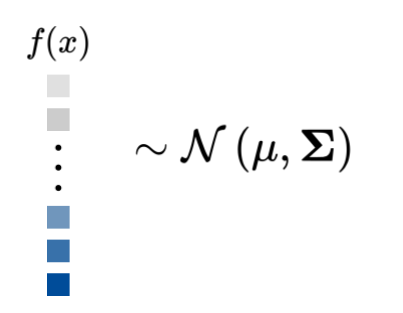
\includegraphics[width=0.5\textwidth]{figure_man/discrete/marginalization-more.png}}
      \only<4>{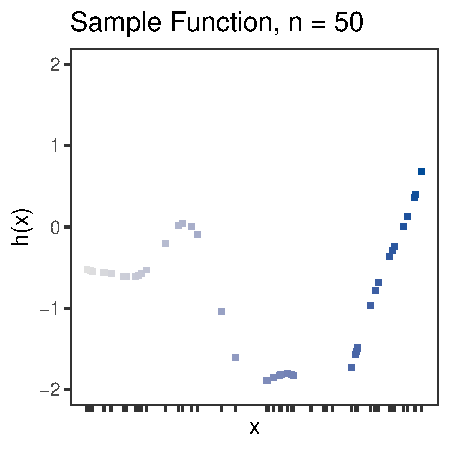
\includegraphics[width=0.4\textwidth]{figure_man/discrete/example_marginalization_50.pdf}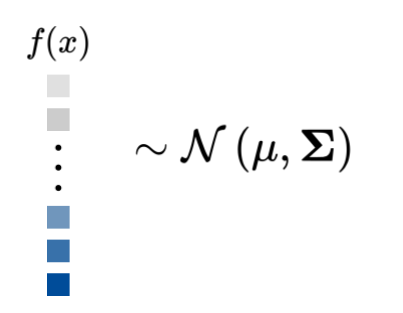
\includegraphics[width=0.5\textwidth]{figure_man/discrete/marginalization-more.png}}
   \end{figure}
    }
\end{itemize}

\end{frame}


\begin{vbframe}{Gaussian Processes}

This intuitive explanation is formally defined as follows: 

\lz 

A function $\fx$ is generated by a GP $\gp$ if for \textbf{any finite} set of inputs $\left\{\xv^{(1)}, \dots, \xv^{(n)}\right\}$, the associated vector of function values $\bm{f} = \left(f(\xv^{(1)}), \dots, f(\xv^{(n)})\right)$ has a Gaussian distribution

$$
\bm{f} = \left[f\left(\xi[1]\right),\dots, f\left(\xi[n]\right)\right] \sim \mathcal{N}\left(\bm{m}, \bm{K}\right),
$$

with 


\begin{eqnarray*}
\textbf{m} &:=& \left(m\left(\xi\right)\right)_{i}, \quad
\textbf{K} := \left(k\left(\xi, \xv^{(j)}\right)\right)_{i,j}, 
\end{eqnarray*}
 
where $m(\xv)$ is called mean function and $k(\xv, \xv^\prime)$ is called covariance function. 


\framebreak 

\vspace*{0.5cm} 

A GP is thus \textbf{completely specified} by its mean and covariance function

\vspace*{-0.2cm}
\begin{eqnarray*}
m(\xv) &=& \E[f(\xv)] \\
k(\xv, \xv^\prime) &=& \E\biggl[\left( f(\xv) - \E[f(\xv)] \right) \left( f(\xv^\prime) - \E[f(\xv^\prime)] \right)\biggr]
\end{eqnarray*}

\vfill

\textbf{Note}: For now, we assume $m(\xv) \equiv 0$. This is not necessarily a drastic limitation - thus it is common to consider GPs with a zero mean function. 

% \framebreak

% \vspace*{0.5cm}

% Intuitively, one can think of a function $f$ drawn from a Gaussian process prior as a Gaussian distribution with an \enquote{infinitely} long mean vector and an \enquote{infinite by infinite} covariance matrix.

% \lz

% Each dimension of the Gaussian corresponds to an element $\xv$ from the domain $\mathcal{X}$. The corresponding component of the random vector represents the value of $f(\xv)$.

% \lz

% The \textbf{marginalization property} makes it possible to handle this \enquote{infinite} representation: evaluations of the process on any finite number of points follow a multivariate normal distribution.

\end{vbframe}

\begin{vbframe}{Sampling from a Gaussian process Prior}

We can draw functions from a Gaussian process prior. Let us consider $\fx \sim \mathcal{GP}\left(0, k(\xv, \xv^\prime)\right)$ with the squared exponential covariance function $^{(*)}$

$$
k(\xv, \xv^\prime) = \exp\left(-\frac{1}{2\ls^2}\|\xv - \xv^\prime\|^2\right), ~~ \ls = 1.
$$
\vspace{-4cm}
This specifies the Gaussian process completely. 

\vspace{8cm}
\footnotesize
$^{(*)}$ We will talk later about different choices of covariance functions. 

\normalsize

\framebreak 

To visualize a sample function, we 

\begin{itemize}
  \item choose a high number $n$ (equidistant) points $\left\{\xv^{(1)}, \dots, \xv^{(n)}\right\}$
  \item compute the corresponding covariance matrix $\Kmat = \left(k\left(\xi, \xv^{(j)}\right)\right)_{i,j}$ by plugging in all pairs $\xv^{(i)}, \xv^{(j)}$ 
  \item sample from a Gaussian $\bm{f} \sim \mathcal{N}(\bm{0}, \bm{K})$. 
\end{itemize}

We draw $10$ times from the Gaussian, to get $10$ different samples.  

% Using $100$ equidistant points, we repeat the process of generating the Gaussian $10$ times ($10$ different functions) and draw each function by connecting the sampled values. 

% \lz

\begin{figure}
  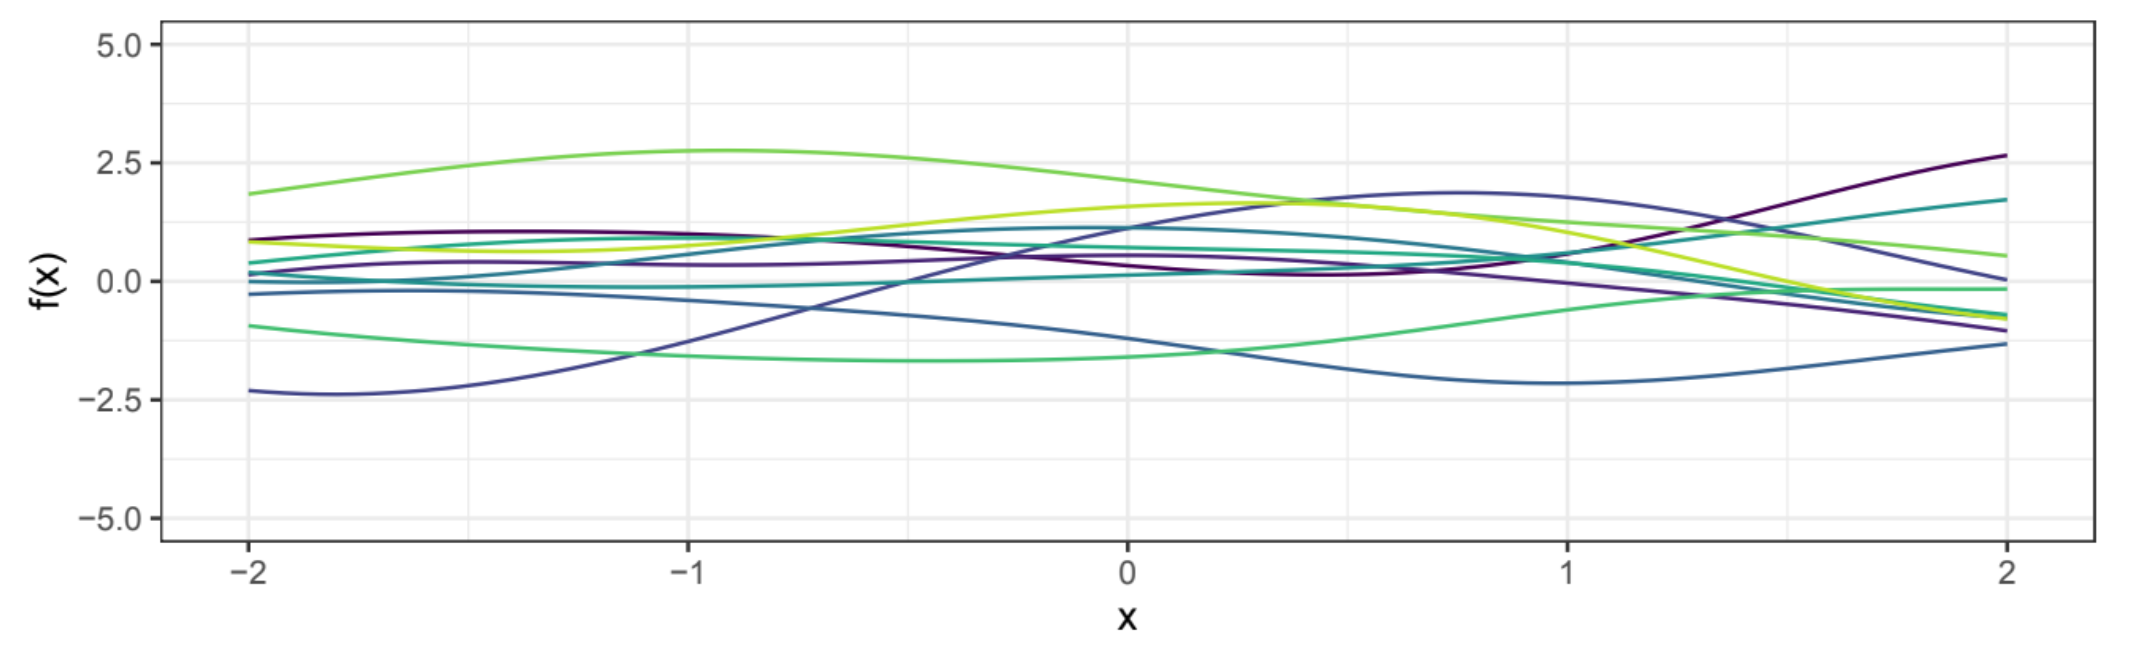
\includegraphics[width=0.9\textwidth]{figure_man/different-samples.png}
\end{figure}

\vspace{-0.2cm}
Since we specified the mean function to be zero $m(\xv) \equiv 0$, the drawn functions have zero mean.

\end{vbframe}


\section{Gaussian Processes as Indexed Family}




\begin{vbframe}{Gaussian processes as an Indexed Family}

% \begin{block}{Definition}
% A \textbf{Gaussian process} is a (infinite) collection of random variables, any \textbf{finite} number of which have a \textbf{joint Gaussian distribution}.
% \end{block}

% \lz

A Gaussian process is a special case of a \textbf{stochastic process} which is defined as a collection of random variables indexed by some index set (also called an \textbf{indexed family}). What does it mean? 

\lz 

An \textbf{indexed family} is a mathematical function (or \enquote{rule}) to map indices $t \in T$ to objects in $\mathcal{S}$. 

\begin{block}{Definition}
A \textbf{family of elements in $\mathcal{S}$ indexed by $T$} (indexed family) is a surjective function 
\vspace*{-0.3cm}
\begin{eqnarray*}
s: T &\to& \mathcal{S} \\
   t &\mapsto& s_t = s(t) 
\end{eqnarray*}
\end{block}

\end{vbframe}

\begin{vbframe}{Indexed Family}

Some simple examples for indexed families are:

\vspace*{0.3cm}

\begin{minipage}{0.43\linewidth}
  \begin{itemize}
  \item finite sequences (lists): $T = \{1, 2, \dots, n\}$ and $\left(s_t\right)_{t \in T} \in \R$ \vspace{1cm}
  \item infinite sequences: $T = \N$ and $\left(s_t\right)_{t \in T} \in \R$
  \end{itemize}
\end{minipage}
\begin{minipage}{0.55\linewidth}
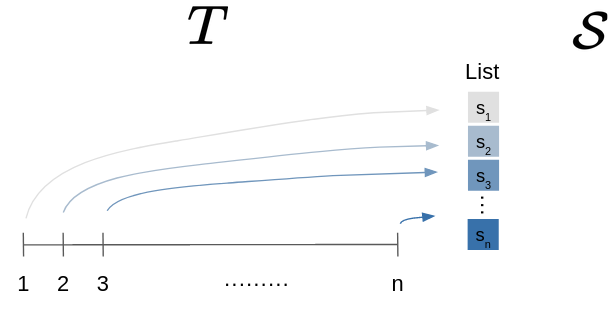
\includegraphics{figure_man/indexed_family/indexed_family_1.png} \\
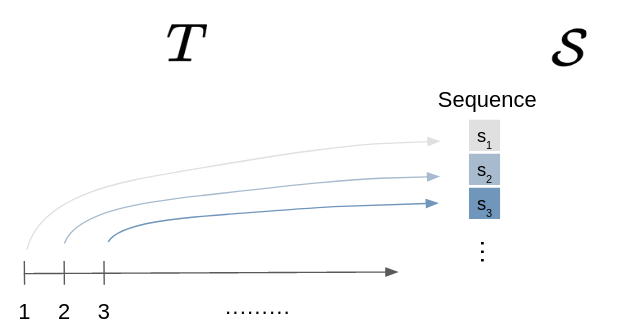
\includegraphics{figure_man/indexed_family/indexed_family_2.png}
\end{minipage}


\framebreak

But the indexed set $\mathcal{S}$ can be something more complicated, for example functions or \textbf{random variables} (RV):

\begin{minipage}{0.43\linewidth}
  \vspace*{0.5cm}
  \begin{itemize}
    \item $T = \{1, \dots, m\}$, $Y_t$'s are RVs: Indexed family is a random vector. \vspace*{0.2cm}
    \item $T = \{1, \dots, m\}$, $Y_t$'s are RVs: Indexed family is a stochastic process in discrete time \vspace*{0.2cm}
    \item $T = \Z^2$, $Y_t$'s are RVs: Indexed family is a 2D-random walk.
  \end{itemize}
\end{minipage}\hfill
\begin{minipage}{0.5\linewidth}
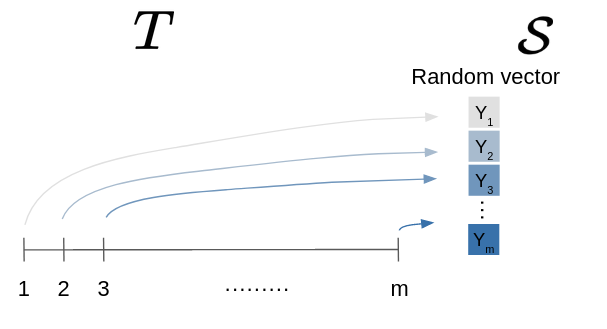
\includegraphics{figure_man/indexed_family/indexed_family_4.png} \\
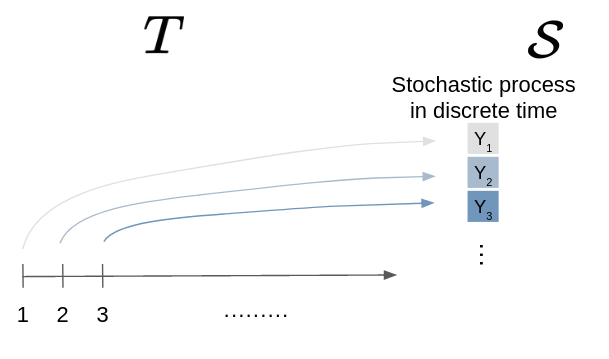
\includegraphics{figure_man/indexed_family/indexed_family_3.png}
\end{minipage}

\end{vbframe}

\begin{frame}{Indexed Family}

\begin{itemize}
  \item A Gaussian process is also an indexed family, where the random variables $f(\xv)$ are indexed by the input values $\xv \in \Xspace$. 
  \item Their special feature: Any indexed (finite) random vector has a multivariate Gaussian distribution (which comes with all the nice properties of Gaussianity!). 
\end{itemize}

\begin{figure}
  \includegraphics<1>[width=0.7\textwidth]{figure_man/indexed_family/indexed_family_5.png} \par
  \only<1>{\begin{footnotesize} Visualization for a one-dimensional $\Xspace$. \end{footnotesize}}
  \includegraphics<2>[width=0.6\textwidth]{figure_man/indexed_family/indexed_family_6.png}\par
  \only<2>{\begin{footnotesize} Visualization for a two-dimensional $\Xspace$. \end{footnotesize}}
\end{figure}

\end{frame}


\endlecture
\end{document}
